\chapter{\IfLanguageName{dutch}{Stand van zaken}{State of the art}}%
\label{ch:stand-van-zaken}
% Tip: Begin elk hoofdstuk met een paragraaf inleiding die beschrijft hoe
% dit hoofdstuk past binnen het geheel van de bachelorproef. Geef in het
% bijzonder aan wat de link is met het vorige en volgende hoofdstuk.

% Pas na deze inleidende paragraaf komt de eerste sectiehoofding.

% Dit hoofdstuk bevat je literatuurstudie. De inhoud gaat verder op de inleiding, maar zal het onderwerp van de bachelorproef *diepgaand* uitspitten. De bedoeling is dat de lezer na lezing van dit hoofdstuk helemaal op de hoogte is van de huidige stand van zaken (state-of-the-art) in het onderzoeksdomein. Iemand die niet vertrouwd is met het onderwerp, weet nu voldoende om de rest van het verhaal te kunnen volgen, zonder dat die er nog andere informatie moet over opzoeken \autocite{Pollefliet2011}.

% Je verwijst bij elke bewering die je doet, vakterm die je introduceert, enz.\ naar je bronnen. In \LaTeX{} kan dat met het commando \texttt{$\backslash${textcite\{\}}} of \texttt{$\backslash${autocite\{\}}}. Als argument van het commando geef je de ``sleutel'' van een ``record'' in een bibliografische databank in het Bib\LaTeX{}-formaat (een tekstbestand). Als je expliciet naar de auteur verwijst in de zin (narratieve referentie), gebruik je \texttt{$\backslash${}textcite\{\}}. Soms is de auteursnaam niet expliciet een onderdeel van de zin, dan gebruik je \texttt{$\backslash${}autocite\{\}} (referentie tussen haakjes). Dit gebruik je bv.~bij een citaat, of om in het bijschrift van een overgenomen afbeelding, broncode, tabel, enz. te verwijzen naar de bron. In de volgende paragraaf een voorbeeld van elk.

% \textcite{Knuth1998} schreef een van de standaardwerken over sorteer- en zoekalgoritmen. Experten zijn het erover eens dat cloud computing een interessante opportuniteit vormen, zowel voor gebruikers als voor dienstverleners op vlak van informatietechnologie~\autocite{Creeger2009}.

% Let er ook op: het \texttt{cite}-commando voor de punt, dus binnen de zin. Je verwijst meteen naar een bron in de eerste zin die erop gebaseerd is, dus niet pas op het einde van een paragraaf.
\section{Technische specificaties}
In dit eerste hoofdstuk worden de technische specificaties besproken van de verschillende technologieën die in deze bachelorproef gebruikt worden.
Er wordt dieper ingegaan op het gebruik van Cosmos DB, NodeJS, de Gremlin API en de verschillende AI-modellen die ingezet worden om de data te bevragen en te analyseren.
Daarnaast worden ook andere technische mogelijkheden besproken die getest zijn, maar uiteindelijk niet gebruikt werden, inclusief de bijbehorende redenen.

\subsection{Grafiekmodellering}
Grafiekmodellering is een techniek die gebruikt wordt om de data te visualiseren en te analyseren~\autocite{neo4j20252}.
Deze data wordt opgeslagen in een grafiekdatabase zoals Cosmos DB~\autocite{Azure2024}. 
In deze bachelorproef wordt grafiekmodellering gebruikt om de verbanden te leggen tussen de verschillende processen binnen ArcelorMittal Gent.
Dit gebeurt doordat één of meerdere knopen verbonden zijn met andere knopen door middel van een relatie.
Een knoop stelt een entiteit voor, zoals een persoon, een product of een proces. 
Een verbinding stelt de relatie tussen de verschillende knopen voor, zoals een \emph{associatie}, \emph{transformatie} of \emph{transactie} van een product~\autocite{Byun2020}.
Dit kan in ons geval een kraan zijn die verbonden is met een machine. Hierbij zijn de kraan en de machine de knopen en is de relatie een \emph{associatie} tussen deze knopen.

Om de traceerbaarheid te behouden wordt bij het wijzigen van een knoop ook de tijdstempel opgeslagen van deze wijziging, zodat er altijd kan worden opgevraagd wanneer deze knoop is gewijzigd.
De relatie zal in dit geval worden omgezet naar een ``has-event''-relatie die een ``delete event'' eigenschap bevat, zegt~\autocite{Byun2020}.
Deze ``delete'' wordt gedaan door de knopen van uitgaande relaties op te slaan, de huidige relatie te verwijderen en een nieuwe relatie toe te voegen met elke opgeslagen uitgaande knoop.

Elke knoop bevat ook eigenschappen die zichzelf beschrijven, zoals het bouwjaar, het laatste onderhoud of zelfs sensordata, zoals een alarm op de machine.
Deze data wordt opgeslagen als sleutel-waarde paren om dit later efficiënt te kunnen ophalen, door in de query te vragen naar de sleutel en de waarde.
In figuur~\ref{fig:graphmodel} is een voorbeeld te zien van een grafiekmodel met fictieve data dat opgezet is in Cosmos DB.\@
Daarnaast is er in schema~\ref{fig:chatbot_workflow} een visuele voorstelling van de workflow van de chatbot die is opgezet.

\begin{figure}[H]
     \centering
     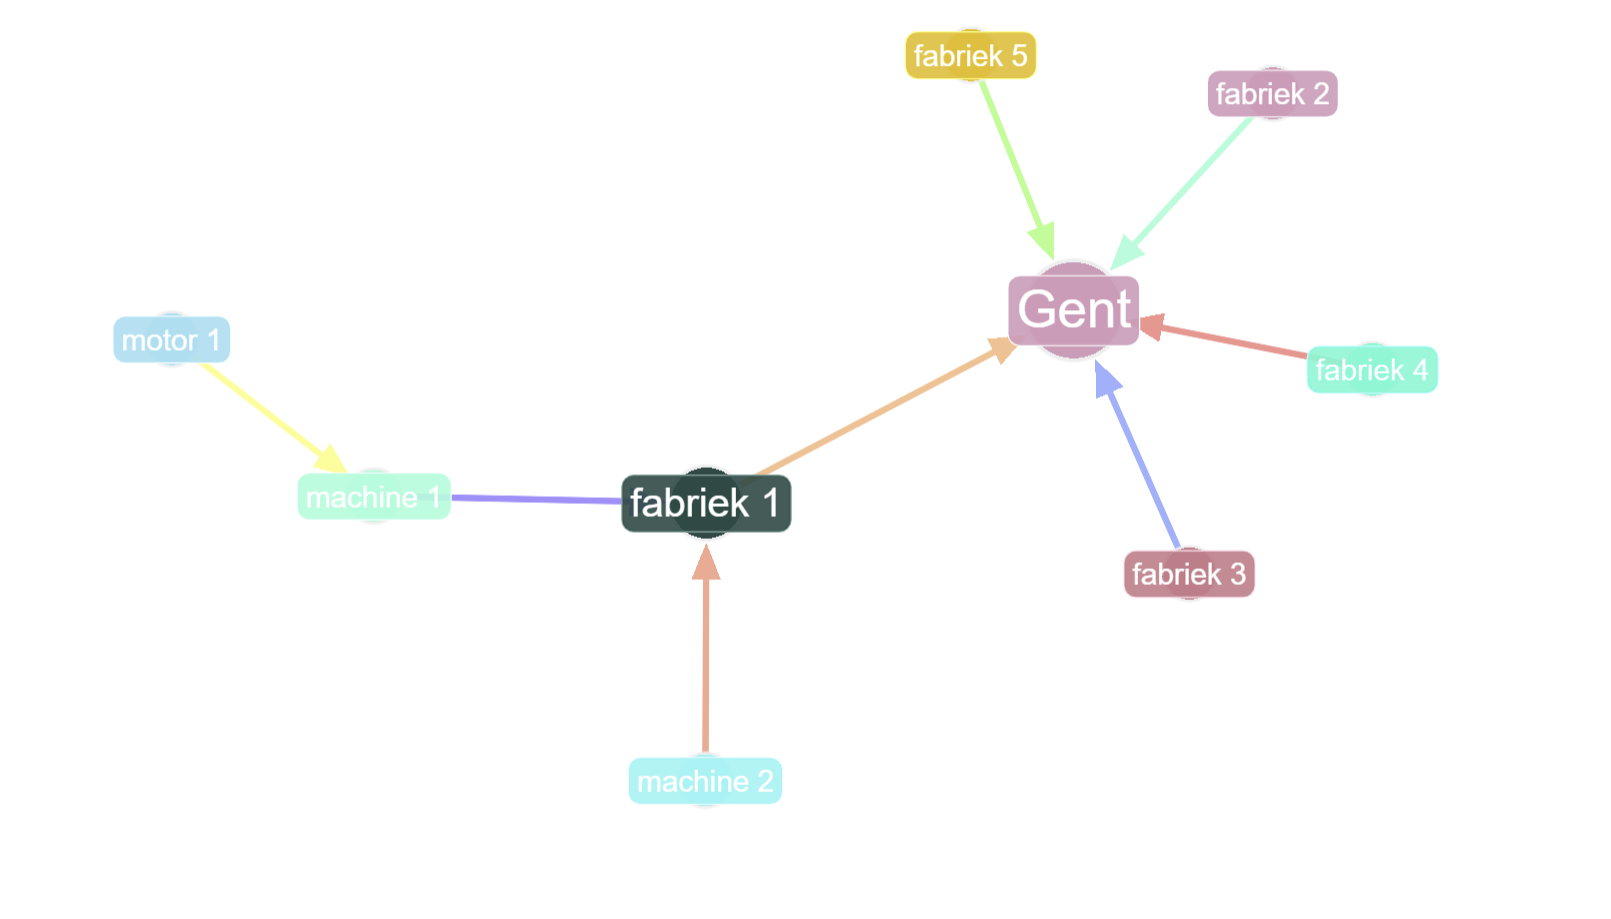
\includegraphics[width=0.8\textwidth]{./img/grapmodel_example.png}
     \caption[Voorbeeld Grafiekmodel.]{\label{fig:graphmodel}Voorbeeld van kleinschalig grafiekmodel, gemaakt met mock data.}
\end{figure}

\subsection{Cosmos DB}
Cosmos DB is een NoSQL-database van het Microsoft Azure-ecosysteem. Het biedt een lage latentie, is beschikbaar voor verschillende API's en kan grote hoeveelheden data verwerken met een hoge beschikbaarheid, wat belangrijk is in ons project~\autocite{CosmosDB2024}.
Daarnaast is Cosmos DB horizontaal schaalbaar, wat betekent dat er op piekmomenten tot een miljoen lees- en schrijfaanvragen verwerkt kunnen worden door het benodigde aantal servers toe te voegen.
De hoge beschikbaarheid wordt gegarandeerd door replicatie, waardoor er snel kan worden overgeschakeld als er een probleem is in onze database.

Binnen ArcelorMittal wordt gebruikgemaakt van onder andere de Azure-omgeving van Microsoft, waardoor Cosmos DB een logische keuze is voor ons project.
Cosmos DB ondersteunt verschillende API's zoals SQL, MongoDB, Cassandra, Gremlin en Table API, waardoor er flexibel kan worden gewerkt met verschillende soorten data.

In deze thesis wordt gebruikgemaakt van Cosmos DB, omdat dit een grafiekdatabase bevat die ons in staat stelt om de data te structureren en te doorzoeken op basis van de relaties tussen de verschillende knopen.
Om op een later moment verbanden te kunnen leggen tussen processen binnen ArcelorMittal Gent, is dit onderdeel noodzakelijk voor het project.

Om de query's uit te voeren op Cosmos DB wordt gebruikgemaakt van de Gremlin API, wat later uitgebreid wordt besproken in~\ref{sec:gremlin}.
Voor deze thesis is er gebruikgemaakt van Cosmos DB, die een \emph{free tier} heeft met een beperkte hoeveelheid Request Units (RU's) per seconde.
Dit is een gratis versie van Cosmos DB die verkrijgbaar is via het studenten-abonnement van Microsoft Azure.
In productie zou gebruik worden gemaakt van de betaalde versie van Cosmos DB, die meer Request Units (RU's) per seconde kan verwerken en meer opslagcapaciteit biedt.
In het volgende hoofdstuk gaan we dieper in op hoe de kosten bepaald worden, en welke schaalmodellen beschikbaar zijn.

In codefragment~\ref{fig:gremlinClient} is een voorbeeld te zien van hoe er verbinding wordt gemaakt met de database. Dit gebeurt via de Gremlin API, waarbij er een authenticator gebruikt wordt om verbinding te maken met de database.
Alle configuratiegegevens, zoals de databasenaam, collectienaam, endpoint en primary key, worden opgeslagen in een aparte configuratiefile, zodat deze gemakkelijk kunnen worden aangepast zonder de code te wijzigen.
Door deze functie in een apart script te plaatsen en te exporteren, kan deze functie overal waar het nodig is gebruikt worden in de chatbot.
Dit zorgt er ook voor dat als er iets verandert aan de verbinding met de database, dit slechts op één plaats hoeft te worden aangepast en niet in elke functie die de database gebruikt.

\subsubsection{Request Units (RU)}
Cosmos DB werkt met Request Units (RU's), een abstracte maat voor de hoeveelheid systeembronnen (zoals CPU, geheugen en I/O) die nodig zijn om een bepaalde bewerking of query uit te voeren~\autocite{Brown2024}.
Elke bewerking krijgt een aantal Request Units toegewezen afhankelijk van de complexiteit en de gebruikte API, zegt~\textcite{Brown2024}.

Bij het bekijken van de resource-monitor van de Cosmos Database, werd er voor een query zoals ``Geef alle kranen met een alert op de motor'' ongeveer 10 RU's gerekend.
Voor dit onderzoek is er minder rekening gehouden met de RU's, aangezien er met een kleine dataset gewerkt wordt en de kosten veel lager zullen zijn dan in een productieomgeving.
Daarnaast maakt het aantal gebruikers ook een aanzienlijk verschil in de kosten, wat op dit moment nog niet kan worden ingeschat.
In figuur~\ref{fig:RU} is te zien  hoeveel RU's er gebruikt zijn bij het testen van de chatbot.
Hierbij is te zien dat als er op één dag veel gebruikgemaakt wordt van de chatbot door één persoon, dat er al snel gemiddeld 200 RU's gebruikt worden.
Dit komt voor één regio (bijvoorbeeld Europa) neer op ongeveer 10 tot 15 euro per maand, wat voor grote bedrijven vaak een verwaarloosbaar bedrag is~\autocite{azurePrices25}.
Indien er toch veel rekening gehouden moet worden met de kosten, is het belangrijk om het juiste schaalmodel te kiezen en de juiste overwegingen te maken.

Bij Microsoft Azure zijn er verschillende manieren om te betalen voor verbruik (of RU's) in Cosmos DB, afhankelijk van het benodigde schaalmodel:
\begin{itemize}
     \item Bij provisioned throughput reserveer je een vast aantal Request Units per seconde (RU/s), waarvoor je betaalt ongeacht of je ze volledig gebruikt. Dit model is geschikt voor toepassingen met een constante of voorspelbare belasting~\autocite{provisioned2024}.
     \item Bij serverless throughput betaal je enkel voor het aantal RU's dat effectief verbruikt wordt. Aan het einde van de facturatieperiode wordt het totale verbruik aangerekend. Dit model is ideaal voor sporadisch gebruik of ontwikkelomgevingen met een lage belasting~\autocite{serverless2025}.
     \item Met autoscale throughput stel je een maximumcapaciteit in, waarna Cosmos DB automatisch schaalt tussen 10\% en 100\% van die waarde, afhankelijk van de werkelijke belasting~\autocite{autoscale2024}. Het voordeel van autoscale throughput is dat je geen handmatige schaling hoeft te doen. Een nadeel daarentegen is dat je altijd minimaal 10\% van de ingestelde maximumwaarde betaalt, wat bij lage activiteit duurder kan uitvallen dan het serverless model.
 \end{itemize}

 \begin{figure}[H]
     \centering
     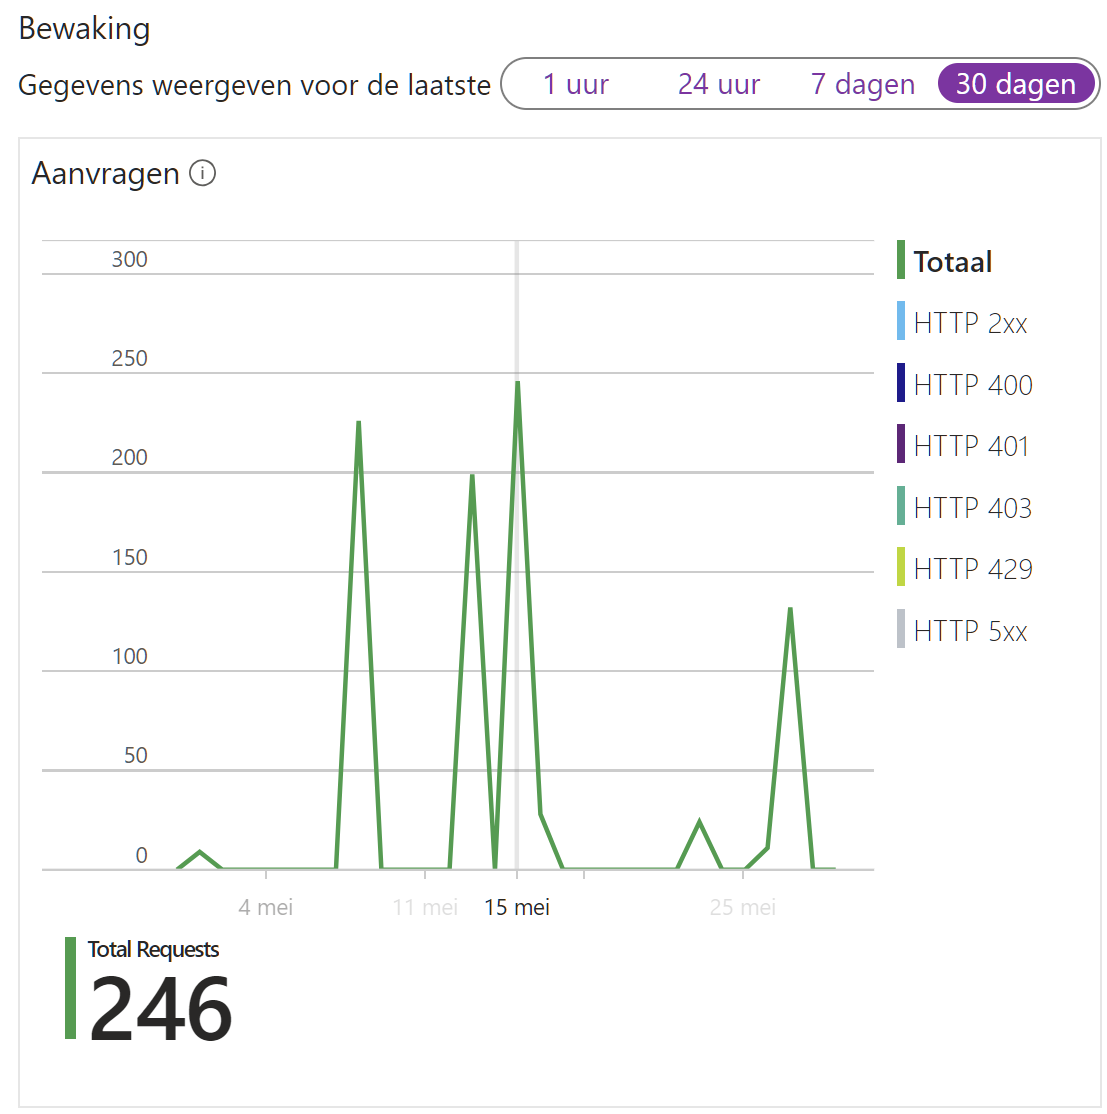
\includegraphics[width=0.6\textwidth]{./img/requestUnits.png}
     \caption[Verbruik Request Units]{\label{fig:RU}Verbruik Request Units één testdag met één persoon.}
\end{figure}

\subsection{API:\@ Apache Gremlin}{\label{sec:gremlin}}
Om ervoor te zorgen dat de data kan worden opgehaald en bevraagd in Cosmos DB, wordt de Gremlin API van Apache TinkerPop gebruikt~\autocite{Tinkerpop2023}.
Apache TinkerPop is een framework voor grafiekberekeningen dat gebruikt wordt voor grafiekdatabases en grafiekanalyses.
Het protocol van Gremlin is gebaseerd op een REST-API die communiceert tussen de database en de chatbot, waardoor er na bevraging een antwoord gegeven wordt met de gegevens uit deze database~\autocite{Medina2021}.

De taal bevat verschillende varianten voor verschillende programmeertalen, zoals Gremlin-Java, Gremlin-Python en Gremlin-Groovy.
In ons geval zal Gremlin-JavaScript gebruikt worden om de data in Cosmos DB te bevragen, aangezien de databaseverbinding via JavaScript geïnitieerd wordt. 
In JavaScript wordt er gebruikgemaakt van de Gremlin client, die de Gremlin API gebruikt om verbinding te maken met de database en de query's uit te voeren.
Een voorbeeld van de Gremlin client is te zien in codefragment~\ref{fig:gremlinClient}.

Hiernaast is ook Neo4J overwogen met Cypher als querytaal, maar deze heeft zijn eigen ecosysteem en is niet even flexibel en schaalbaar als de Gremlin API.\@
Gremlin daarentegen voorziet dat alle databases die TinkerPop-enabled zijn, kunnen gebruikt worden. Dit zijn databases die ondersteund worden door het Apache TinkerPop-framework.
Hieronder vallen onder andere Amazon Neptune, Cosmos DB, JanusGraph en nog vele andere~\autocite{Tinkerpop2023a}.

Via de Gremlin API kunnen verschillende vragen worden gesteld aan de database en wordt de benodigde data opgehaald. 
Zo kan er gevraagd worden welke knopen er zijn, hoeveel uitgaande relaties er zijn, en kan er gezocht worden naar specifieke labels.

Een belangrijke notitie is dat Gremlin case-sensitive is, wat betekent dat de juiste hoofdletters moeten worden gebruikt in de query's.
De hoofdlettergevoeligheid kan er namelijk voor zorgen dat een query niet werkt omdat hij zoekt naar exact het woord.
Hiervoor zijn alle values in de database omgezet naar kleine letters via een klein Python-script, zodat er geen problemen ontstaan bij het ophalen van de data.
Daarnaast zijn er bepaalde sleutelwaarden die in Cosmos DB ook de juiste hoofdletters moeten hebben (zoals \texttt{label} en \texttt{name}), hiervoor is er een kleine lijst meegegeven aan de chatbot die de woorden met de nodige juiste hoofdletters bevat.
Om dit te doen, worden met Python alle keys opgehaald uit de database en opgeslagen in een lijst. Daarna maakt het Large Language Model een query en kijkt het voor elk woord of dit in de lijst aanwezig is.
Indien de string in de lijst staat, wordt de hoofdlettergevoeligheid behouden, anders wordt de string omgezet naar kleine letters.

In codefragment~\ref{fig:gremlin} is een voorbeeld te zien van een Gremlin-query die de knopen verbonden met machine 1 ophaalt.
Zoals te zien in dit codefragment, is er een query voor het opschonen en een query na het opschonen van de hoofdlettergevoeligheid. 
Daarin is te zien dat alles wat in kleine letters moet staan, ook in kleine letters staat.
Hierbij wordt gebruikgemaakt van de \texttt{outE}-functie, die de uitgaande relaties ophaalt van de knoop, en de \texttt{inV}-functie, die de inkomende knopen ophaalt.

\begin{listing} [H]
     \begin{minted}{SQL}
          -- Query voor het opschonen
          g.V().HAS('label', 'MACHINE 1').OUTE('IS_ASSOCIATED').INV()

          -- Query na het opschonen
          g.V().has('label', 'machine 1').outE('is_associated').inV()
     \end{minted}
     \caption[Voorbeeld Gremlin query]{\label{fig:gremlin}Voorbeeld van een Gremlin query die de knopen ophaalt uit de database.}
\end{listing}

\subsection{REST-API}{\label{sec:restapi}}
Om de communicatie tussen de chatbot en de database te voorzien, wordt er gebruikgemaakt van een REST-API, ofwel Representational State Transfer Application Programming Interface~\autocite{RESTAPI2021}.
Een REST-API is een manier om flexibel en lichtgewicht te communiceren tussen verschillende applicaties via HTTP-verzoeken.
Ze maakt gebruik van de CRUD-operaties, oftewel GET, POST, PUT en DELETE, om gegevens op te halen, toe te voegen, bij te werken of te verwijderen.

De REST-architectuur werd voor het eerst ontworpen door Roy Fielding in 2000 en is sindsdien een populaire manier geworden om webservices te bouwen.
Daarnaast is een REST-API ook \emph{stateless}, wat betekent dat elke aanvraag onafhankelijk is van de andere aanvragen en dat er geen informatie wordt opgeslagen tussen sessies.

Voor deze use case wordt gebruikgemaakt van een POST-request waarbij de vraag van een gebruiker wordt doorgegeven.
Als antwoord komt er een JSON-object terug met de resultaten van de query uit de database.
Indien er een knoop of relatie ``verwijderd'' moet worden, moet er een DELETE-request uitgevoerd worden, ook dit is mogelijk via de REST-API.
Als nuance is het belangrijk te vermelden dat een knoop of relatie nooit echt verwijderd wordt, maar enkel gemarkeerd wordt als verwijderd.

Het voordeel van een REST-API is dat deze platformonafhankelijk is en gemakkelijk geïntegreerd kan worden met andere systemen.
Dit komt doordat de requests uitgevoerd worden via HTTP, ofwel Hypertext Transfer Protocol~\autocite{HTTP25}.
Om hier niet te diep op in te gaan, is het belangrijk om te weten dat HTTP een protocol is dat gebruikt wordt om gegevens te verzenden over het internet.

Kort samengevat wordt er een POST-request met de vraag van de gebruiker naar de server verstuurd. Daarna geeft de server een antwoord terug met de resultaten van de query uit de database.
Deze resultaten worden verwerkt door het Large Language Model, dat een samenvatting maakt van de resultaatset en deze terugstuurt naar de gebruiker als een duidelijk, maar beknopt antwoord.

\subsection{Runtime: NodeJS}
NodeJS is een open-source JavaScript-runtimeomgeving die de mogelijkheid biedt om JavaScript-code uit te voeren op een server~\autocite{NodeJS2022}.
Via NodeJS kan een lokale server opgezet worden die de communicatie tussen de chatbot en de database mogelijk maakt.

NodeJS werkt via een \emph{single-threaded, non-blocking I/O}-model, wat betekent dat er geen nieuwe threads worden aangemaakt voor elk verzoek.
Door middel van callbacks en promises werkt NodeJS asynchroon. 
Dit houdt in dat het systeem niet blokkeert terwijl het wacht op bijvoorbeeld een antwoord van de database. 
In plaats daarvan kan de server ondertussen andere taken uitvoeren of verzoeken afhandelen. 
Dit is belangrijk bij deze toepassing, waar grote hoeveelheden data worden verwerkt, zodat het systeem efficiënt blijft en niet onnodig stilvalt tijdens trage bewerkingen zoals grote query's.
Met event loops worden de taken in een wachtrij geplaatst en verwerkt wanneer de server klaar is met een andere operatie.
Daardoor is NodeJS zeer performant en schaalbaar voor het verwerken van grote hoeveelheden data.

De technologie werd in 2009 ontwikkeld en geïntroduceerd door Ryan Dahl en is sindsdien zeer populair geworden binnen de webontwikkeling. 
NodeJS wordt tegenwoordig gebruikt door grote bedrijven zoals Netflix, eBay en Uber voor hun back-end systemen.
Zoals eerder vermeld is het geen framework, maar een runtimeomgeving.

In een schone NodeJS-installatie zijn er slechts een beperkt aantal specifieke modules of bibliotheken aanwezig, waardoor het een zeer lichte en flexibele omgeving is om mee te werken.
De aanwezige modules zijn standaardmodules (core modules), zoals \texttt{http}, \texttt{fs} (file system) en \texttt{path}. 
Deze zorgen voor de basisfunctionaliteit bij het opzetten van een server en het werken met bestanden.
Deze modules zijn vaak nodig om folders en bestanden te beheren, daarom worden ze `standaardmodules' genoemd~\autocite{Kumar2023}.
Naast deze standaardmodules zijn er ook veel externe modules beschikbaar via \texttt{npm} (Node Package Manager), die gebruikt kunnen worden om de functionaliteit van NodeJS uit te breiden.

\subsection{LLM runtime: Ollama}
Om later in deze bachelorproef een chatbot op te bouwen, wordt er gebruikgemaakt van Ollama, een wrapper die het mogelijk maakt om verschillende Large Language Models (LLMs) lokaal te draaien op een server~\autocite{Manandhar2025}. 
Dit is een open-sourcebibliotheek die verschillende vooraf getrainde modellen bevat, zoals de LLaMA-modellen van Meta, de Phi-modellen van Microsoft en nog vele andere.
Naast het gebruik van modellen die standaard beschikbaar zijn via Ollama, is het ook mogelijk om bepaalde Hugging Face-modellen te integreren die lokaal of in een Docker-container kunnen worden opgezet~\autocite{HuggingFace2024}.

Dankzij dit brede aanbod aan bestaande pretrained modellen kunnen er snel vergelijkingen worden gemaakt door eenvoudig nieuwe modellen op te halen via Ollama.
Dit is een groot voordeel, aangezien de scope van deze thesis niet ligt bij het volledig ontwikkelen of trainen van een eigen LLM voor natuurlijke taalverwerking of het genereren van Gremlin-query's.
Wel wordt er gezocht naar het meest geschikte bestaande model voor deze taken, eventueel aangevuld met finetuning. 
Dat vormt echter een uitdaging, omdat er verschillende versies van Gremlin bestaan met afwijkende querysyntaxis, en omdat er momenteel geen gespecialiseerde modellen beschikbaar zijn voor het genereren van Gremlin-query's.
Met behulp van Retrieval-Augmented Generation (RAG) en Elasticsearch wordt dit probleem deels ondervangen. In hoofdstuk~\ref{sec:chatbot} wordt hier dieper op ingegaan.

Tijdens de testfase zijn meerdere modellen geëvalueerd, waaronder LLaMA, CodeLLaMA en Phi-4.
De LLaMA-modellen (LLaMA2 en LLaMA3) bleken redelijk goed in het omzetten van databankgegevens naar natuurlijke taal, maar hadden moeite met het genereren van correcte Gremlin-query's.
CodeLLaMA gaf, mits de nodige finetuning, vaak betere resultaten bij het genereren van deze query's, maar bleek minder sterk in het formuleren van natuurlijke antwoorden op basis van de verkregen data.
Over het algemeen blijft het een uitdaging om Gremlin-query's te genereren met een LLM, omdat deze modellen niet specifiek getraind zijn op de syntaxis van Gremlin.
In sectie~\ref{sec:LORA} wordt een methode besproken waarmee een model kan worden gefinetuned op Gremlin-syntaxis, maar dit is niet verder onderzocht binnen deze thesis wegens beperkte rekenkracht en tijd.

Tot slot werd ook Phi-4 getest, een model ontwikkeld door Microsoft. Dit model is performanter (en dus sneller) dan de LLaMA-modellen, en gaat efficiënt om met de verkregen input.
In het volgende hoofdstuk wordt dieper ingegaan op de geteste modellen, hun prestaties en de uiteindelijke keuze voor een combinatie van twee verschillende modellen.

\subsubsection{Llama2}
LLaMA 2 is een open-source Large Language Model ontwikkeld door Meta AI~\autocite{llama2}. 
Het model is beschikbaar in verschillende versies, met groottes variërend van 7 tot 70 miljard parameters, afhankelijk van de gekozen configuratie.
LLaMA 2 werd ontwikkeld om te concurreren met andere geavanceerde taalmodellen zoals GPT-3.5 en GPT-4.
De training van het model is gebaseerd op een combinatie van supervised finetuning en reinforcement learning met menselijke feedback (RLHF).
Net als bij andere LLMs blijven uitdagingen zoals hallucinaties en bias aanwezig, en kunnen deze tijdens gebruik blijven optreden.

\subsubsection{Llama3}
LLaMA 3 is de opvolger van LLaMA 2 en vormt een state-of-the-art Large Language Model ontwikkeld door Meta AI~\autocite{Meta2024}. 
Met \emph{state-of-the-art} wordt bedoeld dat het model gebruikmaakt van de nieuwste technieken en algoritmes om de prestaties te optimaliseren.
LLaMA 3 bevat verschillende verbeteringen ten opzichte van zijn voorganger, waaronder een grotere trainingsdataset en een verfijnde architectuur.
Net als LLaMA 2 is ook dit model beschikbaar in verschillende versies, met parametergroottes variërend van 7 tot 70 miljard, afhankelijk van de gekozen configuratie.

Daarnaast toont LLaMA 3 licht verbeterde codeerprestaties, bijvoorbeeld bij het genereren van Python- of JavaScript-code. 
Uit onze testen bleek echter dat het model, net als zijn voorgangers, moeite blijft hebben met het genereren van correcte Gremlin-query's.
Hoewel LLaMA 3 op sommige vlakken even goed of zelfs beter presteert dan Phi-4, blijkt uit grafiek~\ref{fig:MMLU} dat het model voor vergelijkbare antwoordkwaliteit ongeveer vijf keer groter is dan Phi-4.
Hierdoor is het model aanzienlijk zwaarder en trager, wat het minder geschikt maakt voor implementatie binnen dit project.

\subsubsection{Phi-4}{\label{sec:phi4}}
Phi-4 is een state-of-the-art Large Language Model ontwikkeld door Microsoft en bevat 14 miljard parameters~\autocite{Kamar2024}. 
Het model is ontworpen als een compact, maar krachtig en performant alternatief dat kan concurreren met grotere modellen zoals LLaMA 3, zoals eerder besproken.
Uit de uitgevoerde testen bleek dat Phi-4 over het algemeen sneller werkt en sterke prestaties levert op het gebied van natuurlijke taalverwerking, in vergelijking met andere omvangrijke modellen.

Figuur~\ref{fig:MMLU} toont de resultaten van de MMLU-benchmark (Massive Multitask Language Understanding), een benchmark die de prestaties van taalmodellen test op verschillende domeinen zoals programmeren, wiskunde en taal.
Uit deze figuur blijkt dat Phi-4 een hoge score behaalt die vergelijkbaar is met het zwaarste model uit de LLaMA 3-reeks.
Dit maakt Phi-4 in deze context bijzonder geschikt: het biedt sterke prestaties binnen een lichtgewicht configuratie, wat cruciaal is in toepassingen waar snelheid en efficiëntie van belang zijn.

Binnen dit project wordt gebruikgemaakt van de 14 miljard parameters tellende, gekwantiseerde versie van Phi-4.
Een gekwantiseerd model is geoptimaliseerd voor lagere geheugengebruik en rekencapaciteit, met slechts een minimale en doorgaans verwaarloosbare impact op de nauwkeurigheid van de gegenereerde tekst~\autocite{Qdrant25}.

Volgens \textcite{microsoft2024phi4} is Phi-4 goed inzetbaar in chatbottoepassingen, onder andere dankzij de mogelijkheid tot eenvoudige finetuning en contextuele aanpassingen.
Het model is in staat om instructies en context op te nemen, bijvoorbeeld via prompt-injectie zoals: 
\textit{``Je bent een expert in het beantwoorden van vragen over Cosmos DB.\@ De belangrijkste informatie die je kan gebruiken staat in het \texttt{items} object van de JSON-response.''}
Dankzij de ondersteuning voor meer dan 40 talen kan deze context ook in het Nederlands worden opgegeven, hoewel de hoogste prestaties doorgaans in het Engels worden behaald.
Toch zijn de resultaten in het Nederlands zeer goed: de antwoorden zijn grammaticaal correct, bevatten accurate samenvattingen van de data, en klinken professioneel en gepast voor de beoogde bedrijfsomgeving.

Om die reden wordt Phi-4 in dit project gebruikt voor het interpreteren van de resultaten uit de JSON-response en het genereren van natuurlijke, beknopte en duidelijke antwoorden naar de gebruiker toe.

\begin{figure}[H]
     \centering
     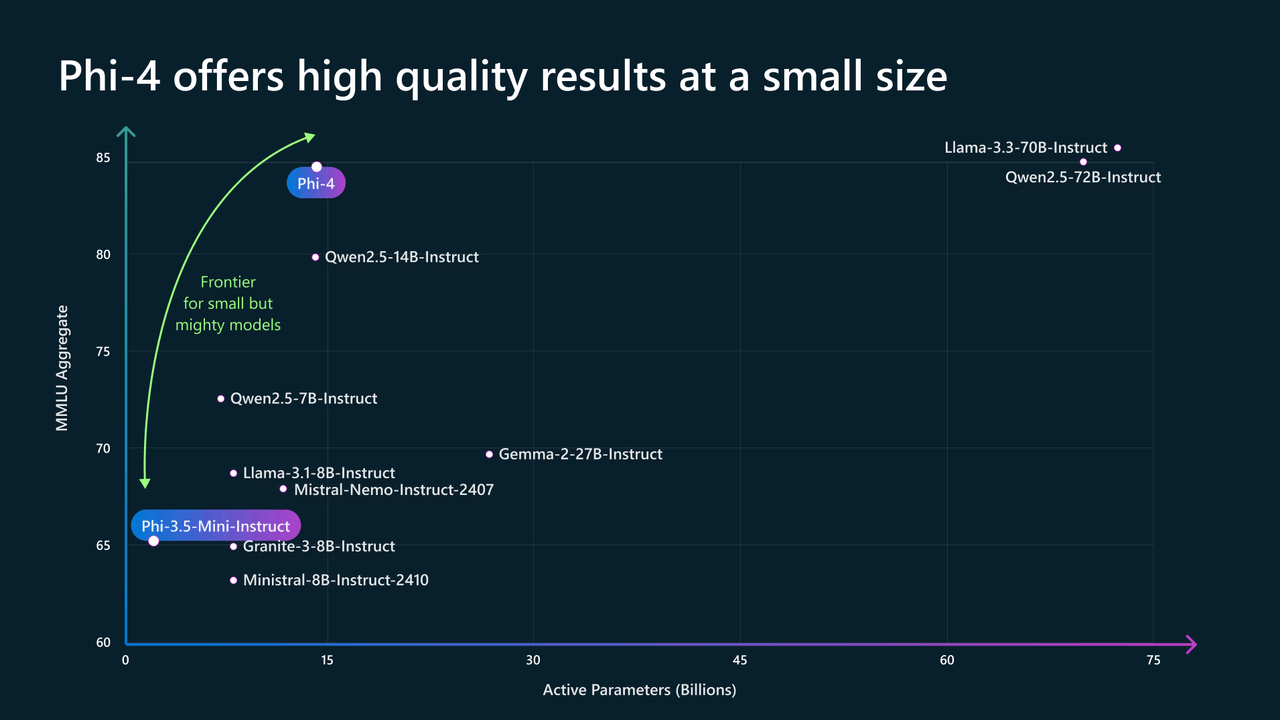
\includegraphics[width=0.8\textwidth]{./img/MMLU.png}
     \caption[benchmark LLMs.]{\label{fig:MMLU}Benchmark verschillende LLMs op de MMLU benchmark.}
\end{figure}

\subsubsection{CodeLLaMA}
Naast de LLaMA-modellen en Phi-4 is ook CodeLLaMA getest. Dit is een open-source model ontwikkeld door Meta AI, specifiek ontworpen voor het genereren en begrijpen van code~\autocite{codellama}. 
Het model is getraind op verschillende programmeertalen zoals Python, JavaScript, C++ en vele anderen. Hierdoor ligt het gebruik van CodeLLaMA voor het genereren van Gremlin-query's voor de hand.

CodeLLaMA is in staat om beter te redeneren en functiekettingen te construeren, wat essentieel is bij Gremlin-query's. Dit wordt mede mogelijk gemaakt door de uitgebreide training op diverse programmeertalen. 
Functiekettingen verwijzen naar het opvolgend aanroepen van verschillende functies binnen een query, zoals \texttt{V()} om knopen op te halen, en \texttt{has()} om te filteren op specifieke sleutel-waardeparen. 
Een voorbeeld hiervan is te vinden in codefragment~\ref{fig:gremlin}.

Door voorbeeldquery's in een JSON-bestand aan het model mee te geven, kan CodeLLaMA de logica van SQL-query's vertalen naar vergelijkbare Gremlin-structuren. 
In deze thesis is gekozen voor een JSON-bestand omdat dit een duidelijke en eenvoudig te begrijpen structuur biedt om query's vast te leggen. 
Oorspronkelijk werd een CSV-bestand gebruikt, maar dit bleek foutgevoelig te zijn door problemen zoals onjuiste aanhalingstekens en onbedoelde kolomsplitsingen door komma's.
JSON voorkomt deze problemen doordat het data als objecten met sleutel-waardeparen opslaat. 
In plaats van aparte kolommen voor vraag en antwoord bevat het JSON-object deze als gekoppelde sleutel-waardeparen. 
Een voorbeeld hiervan is te zien in codefragment~\ref{fig:RAGJSON}.

Hoewel CodeLLaMA sterk is in het genereren van code, is het model minder geschikt voor het beantwoorden van vragen in natuurlijke taal, de antwoorden zijn vaak (grammaticaal) slecht geformuleerd. 
Het model bestaat in verschillende groottes, variërend van 7 tot 70 miljard parameters, en kent diverse versies, zoals gekwantiseerde en instructiemodellen~\autocite{HuggingFaceCodellama}. 
De gekwantiseerde versie is geoptimaliseerd voor snelheid en geheugen, met een lichte daling in nauwkeurigheid, terwijl de instructieversie beter is in het opvolgen van opdrachten en het ondersteunen van programmeertaken.

In dit project wordt gebruikgemaakt van de 7 miljard parameters, gekwantiseerde instructieversie van CodeLLaMA. 
Deze versie is lichtgewicht, kan instructies goed opvolgen, en zorgt voor minimale prestatieproblemen. 
Met instructies wordt bedoeld dat het model beter omgaat met het begrijpen van de vragen en opdrachten. 
CodeLLaMA wordt alleen gebruikt voor het genereren van Gremlin-query's. 
De analyse en interpretatie van de opgehaalde data wordt vervolgens uitgevoerd door Phi-4, dat lichter en sneller is in het genereren van natuurlijke taalantwoorden.

\begin{listing} [H]
     \begin{minted}{js}
          {
               "vraag": "Geef alle motoren",
               "antwoord": "g.V().has('name', containing('motor'))"
          },
     \end{minted}
     \caption[Voorbeeld van een JSON context bestand]{\label{fig:RAGJSON}Voorbeeld JSON met vraag en query.}
\end{listing} 

\subsection{Low Rank Adaptation (LoRA)}{\label{sec:LORA}}
Low Rank Adaptation (LoRA) is een techniek die het mogelijk maakt om grote taalmodellen te finetunen met een beperkte hoeveelheid data~\autocite{Cloudflare}. 
Aan het begin van deze thesis zijn verschillende modellen besproken, zoals Phi-4 en CodeLLaMA, die gebruikt worden voor het verwerken van natuurlijke taal en het omzetten van gebruikersvragen naar Gremlin-query's. 
Gremlin is echter een zeer specifieke taal, die door de verschillende versies en syntaxisvariaties niet altijd eenvoudig automatisch gegenereerd kan worden.

Met behulp van LoRA zoud een oplossing mogelijk zijn door kleine, gerichte aanpassingen toe te voegen aan een bestaand model via een instructiedataset. 
Een machine learning-model bestaat namelijk uit een combinatie van een algoritme en een dataset. 
In het geval van LoRA worden de originele modelgewichten bevroren en worden er extra, low-rank matrices toegevoegd aan deze gewichten door middel van matrixdecompositie~\autocite{Thiyagarajan2024}. 
Deze techniek maakt het mogelijk om efficiënt en met relatief weinig data het model aan te passen. 
Figuur~\ref{fig:lora} toont een voorbeeld van hoe deze matrixdecompositie werkt.

LoRA is een veelbelovende techniek die in toekomstige onderzoeken gebruikt kan worden om de prestaties van de chatbot aanzienlijk te verbeteren. 
Vanwege beperkte beschikbare tijd en resources is deze techniek nog niet geïmplementeerd in de huidige proof of concept van deze thesis.

\begin{figure}[H]
     \centering
     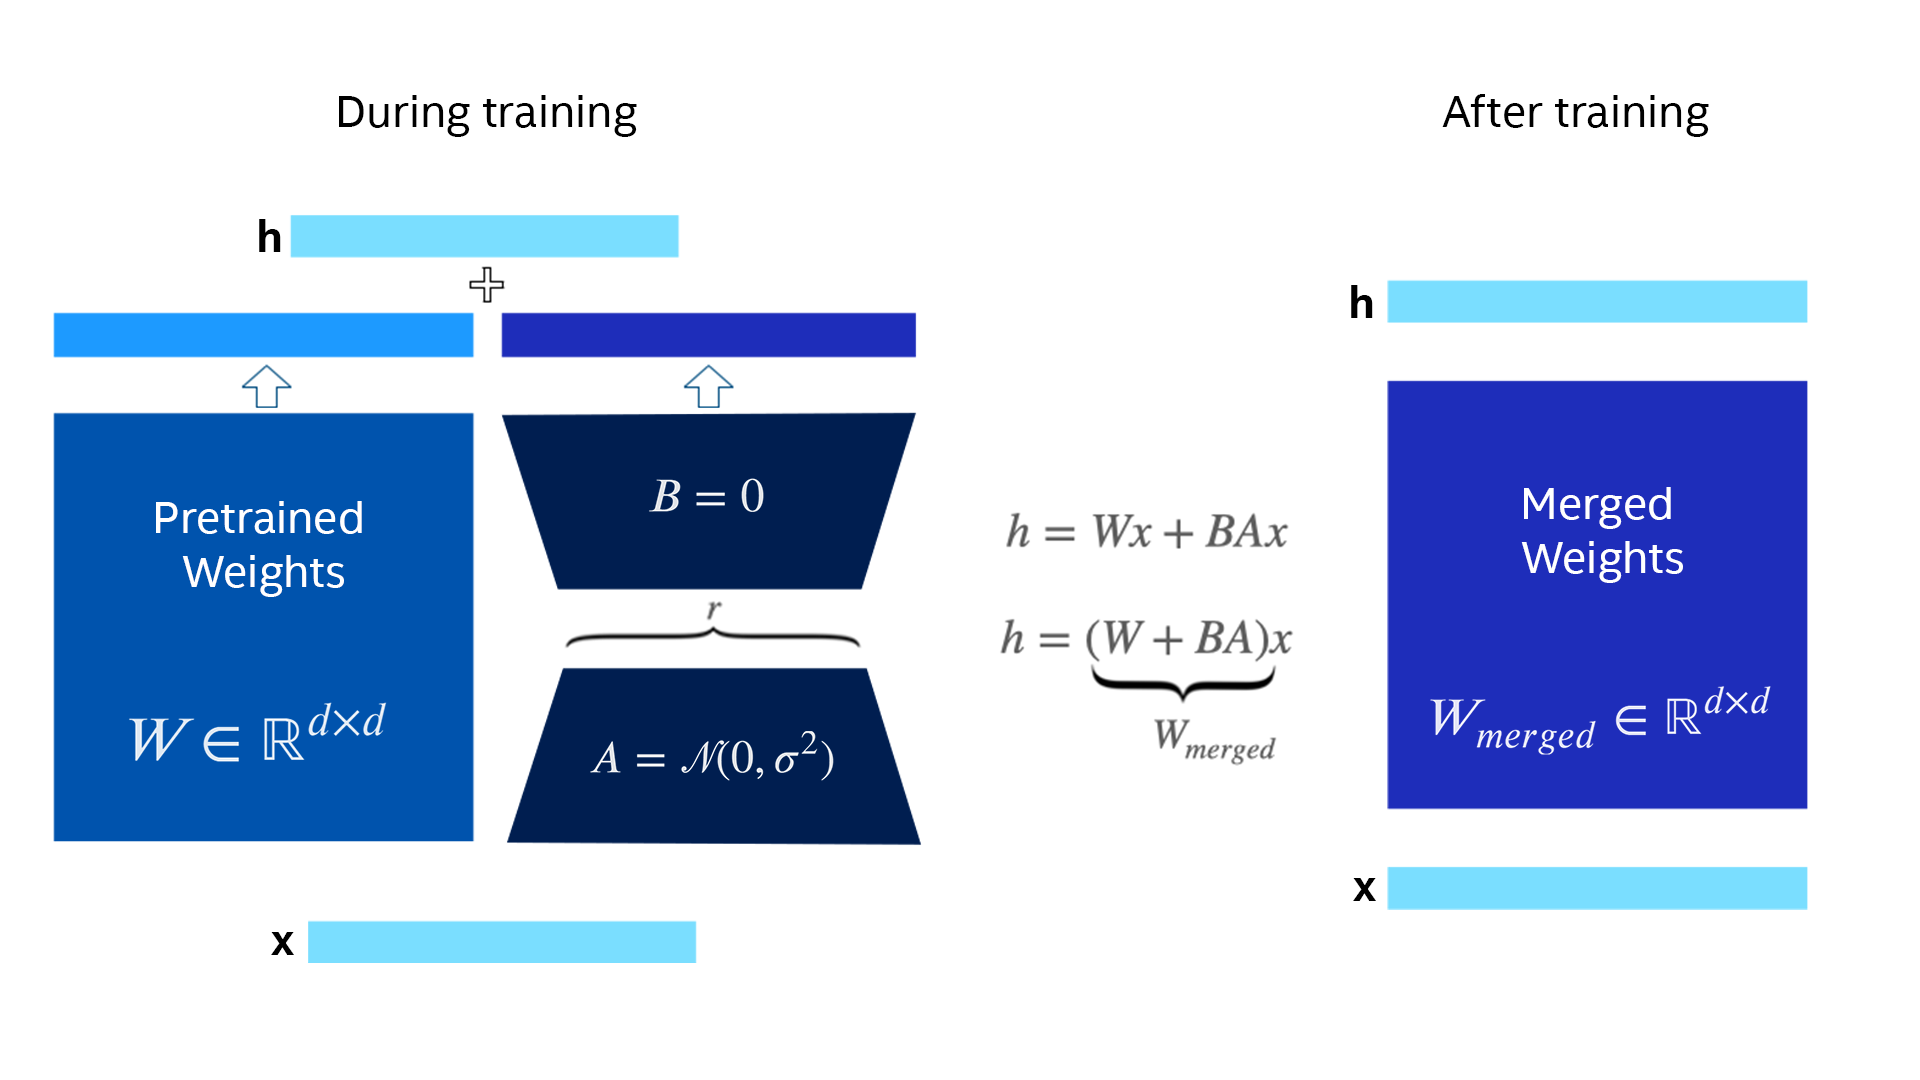
\includegraphics[width=0.8\textwidth]{./img/lora.png}
     \caption[Lora principe.]{\label{fig:lora}Afbeelding waar links pretrained model en rechts merged model is afgebeeld.}
\end{figure}

\section{Data preprocessing}
De data die gebruikt wordt, komt uit een SAP-systeem. Deze data bevat een boomstructuur van de installatie op verschillende levels binnen ArcelorMittal Gent.
Dit betekent dat de data in een hiërarchische structuur is opgebouwd, waarbij de verschillende processen met elkaar verbonden zijn.
Voor het ontcijferen van deze data zijn verschillende specialisten binnen ArcelorMittal gecontacteerd die ons hebben geholpen met het vertalen van de sleutel-waardeparen in de JSON.\@
Er is echter een grote moeilijkheid bij de opsplitsing tussen locatie en machine. Doordat de dataset enorm groot is en er soms handmatige aanpassingen gebeuren door werknemers, kan het zijn dat de levels van de hiërarchie niet altijd correct zijn.
Helaas kan er in dit onderzoek geen garantie worden gegeven door ArcelorMittal dat dit volledig klopt. Na een handmatige controle lijkt dit naar schatting voor 90\% van de data te kloppen, maar bij uitgebreidere afdelingen kan dit verschillen.
Dit betekent dat er voor verdere integratie een structurele aanpassing of opschoning van de dataset nodig is.
Om de basis fundamenteel correct te houden, wordt er in de mock-data gewerkt met de volgende hiërarchie:

\begin{itemize}
     \item level 1: de locatie, bijvoorbeeld Gent.
     \item level 2: de verschillende fabrieken.
     \item level 3: de verschillende machines binnen een fabriek.
     \item level 4: de verschillende motoren van een machine.
\end{itemize}

\subsection{JSON}
De ontvangen data is in JSON-formaat, een veelgebruikte indeling voor het opslaan van gestructureerde gegevens.
JSON, of JavaScript Object Notation, is een tekstgebaseerde indeling die makkelijk te lezen en te schrijven is voor mensen en machines \autocite{Erickson2024}.
Doordat dit formaat zo flexibel is, wordt het vaak gebruikt bij web-, data- en softwareapplicaties.
Hoewel JavaScript in de naam van JSON voorkomt, is het een taalonafhankelijk formaat dat ook in andere programmeertalen kan worden gebruikt.
Aangezien wij gebruikmaken van JavaScript en Python, is dit een voordeel.

JSON werkt op basis van sleutel-waardeparen, waarbij de sleutel een unieke naam is die aan een waarde is gekoppeld.
De waarde kan elk type zijn, zoals een string, nummer, boolean of zelfs een ander JSON-object waarin nog sleutel-waardeparen staan.
Hierdoor kan de data makkelijk gestructureerd en opgeslagen worden in een hiërarchische structuur.
JSON-data is al een zeer goed gestructureerd formaat, maar voor onze toepassing moet deze data nog verder gestructureerd worden.
Dit houdt in dat de verschillende JSON-objecten aan elkaar gelinkt moeten worden, zodat het grafiekmodel hieruit kan worden opgebouwd.
Daarvoor wordt JSON-LD gebruikt, een uitbreiding van JSON die het mogelijk maakt om data te structureren en te annoteren met semantische betekenis.
In codefragment~\ref{jsonData} is een voorbeeld te zien van de mock-data die gebruikt wordt in deze thesis.

\begin{listing} [H]
     \begin{minted}{js}
          {
               "id": "1",
               "name": "Machine 1",
               "label": "machine 1",
               "level": 3,
               "parentId": "2",
               "status": "In Use, Alarm"
          }
     \end{minted}
     \caption[Voorbeeld van een JSON-object]{\label{jsonData}Voorbeeld van een JSON-object in de mock-data.}
\end{listing}

\subsection{JSON-LD}
JSON-LD staat voor JavaScript Object Notation for Linked Data. Dit is een uitbreiding van JSON die het mogelijk maakt om data te structureren en te annoteren~\autocite{jsonld.org}.
Het doel van deze Linked Data is om te zorgen dat je kunt beginnen bij één object en van daaruit de embedded links kunt volgen naar een ander object.
Dit is vergelijkbaar met het grafiekmodel, waarbij er ook vanuit een knoop wordt vertrokken en er van daaruit verschillende relaties kunnen worden gevolgd.
In samenwerking met schema.org en GS1 (standaardnormen voor traceringsdata) kan deze data correct gestructureerd, genormeerd en aan elkaar gelinkt worden.
Het principe is hetzelfde, alleen wordt het model hier gecodeerd in een formaat dat makkelijk te lezen en te schrijven is voor mensen.
Daarna kan deze JSON-LD direct worden ingelezen in Cosmos DB om deze links op te slaan en te visualiseren.
Deze links zijn belangrijk, omdat er moet worden gevonden welke knopen aan elkaar verbonden zijn en welke dus invloed op elkaar hebben.

In deze thesis zijn er twee verschillende JSON-LD-bestanden gebruikt, namelijk \texttt{mock\_data.jsonld} en \texttt{mock\_data\_EPCIS.jsonld}.
Dit omdat we op basis van de gewone mock-data de EPCIS-events bepalen, die later in de chatbot gebruikt worden.

Via een JavaScript-script wat dezelfde code als codefragment~\ref{fig:convertjson} bevat, worden deze JSON-LD-bestanden omgezet naar een grafiekmodel.
Eerst worden alle JSON sleutel-waardeparen omgezet naar de sleutel-waardeparen die nodig zijn voor JSON-LD.\@
Zo gebruiken we bij het \texttt{type} de juiste schema.org-types, zoals \texttt{Place} voor locaties en \texttt{Product} voor machines.
Deze \texttt{Place} en \texttt{Product} types worden bepaald aan de hand van het level, zoals eerder besproken.

Er bestaan ook andere formaten zoals PYLD (Python Linked Data), dotNetRDF (.NET Resource Description Framework), \dots. 
Doordat onze omgeving in JavaScript is opgebouwd en JSON-LD goed functioneert met Gremlin, is dit een goede keuze.
Daarnaast zijn veel mensen bekend met JSON, waardoor implementatie en gebruik eenvoudiger zijn met enige technische kennis.

\begin{listing} [H]
     \begin{minted}{js}
          const node = {
                "@id": `am:${id}`,
                "@type": level > 3 ? "Product" : "Place",
                "name": name,
                "label": label || null,
                "containedInPlace": parentId ? `am:${parentId}` : null,
                ...cleanedItem,
            };
            nodes.push(node);
          };
     \end{minted}
     \caption[Voorbeeld van een JSON naar JSON-LD conversie]{\label{fig:convertjson}Voorbeeld van een JSON naar JSON-LD conversie.}
\end{listing}

\subsection{JSON-LD tot Graph}
Om onze JSON-LD om te zetten naar een grafiekmodel wordt gebruikgemaakt van JavaScript, waarbij de connectie wordt gemaakt zoals in ~\ref{fig:gremlinClient} met onze Cosmos DB.\@
Door het gebruik van deze JavaScript-code begint de conversie van JSON-LD naar een grafiekmodel. Mits een goede vertaling van JSON naar JSON-LD is dit een relatief eenvoudige taak.
In figuur~\ref{fig:addData} is een voorbeeld te zien van hoe de JSON-LD wordt omgezet naar een Gremlin-query die de knoop toevoegt aan de database.
Dit wordt gedaan voor elk JSON-LD-object dat wordt opgehaald uit de JSON-LD-bestanden.

In de JSON-LD staat ook de eigenschap \texttt{label}, die wordt gebruikt om de knoop te identificeren.
Hiervoor is ervoor gekozen om het \texttt{ID} als \texttt{label} te gebruiken, dit is een unieke waarde die de knoop identificeert.
Naast het label worden ook andere eigenschappen toegevoegd aan de knoop die relevant zijn, zoals de alarmstatus van de knoop.

\begin{listing} [H]
     \begin{minted}{js}
          const gremlinQuery = `
               g.addV('${label}')
               .property('id', '${id}')
               .property('label', '${label}')
               ${propertiesString}
               `;

          await client.submit(gremlinQuery);
     \end{minted}
     \caption[Voorbeeld van een JSON-LD naar Graph conversie]{\label{fig:addData}Voorbeeld van een JSON-LD naar Graph conversie.}
\end{listing}
\section{Datemodellering en structuur}
\subsection{GS1}
GS1 is een wereldwijde organisatie die standaarden ontwikkelt voor identificatie, codering \& uitwisseling~\autocite{GS1standards}.
Deze standaarden helpen bedrijven om hun producten en diensten te identificeren, traceren en uit te wisselen.
Elk product heeft een unieke identificatiecode, waardoor het mogelijk is het product te traceren doorheen de toeleveringsketen.
GS1 heeft verschillende standaarden ontwikkeld, zoals de GTIN-code (Global Trade Item Number) en de GLN-code (Global Location Number).
De GTIN-code is een code voor producten, elk product dat traceerbaar wil zijn, moet een GTIN-code hebben.
Als de GTIN-code niet aanwezig is, kan het product niet worden geïdentificeerd en zal de fabrikant of leverancier deze moeten aanvragen bij GS1.
Ook locaties kunnen een unieke code krijgen, namelijk de GLN-code. In volgende hoofdstukken wordt dieper ingegaan op de ontwikkeling van de GTIN- en GLN-codes, de rest van de GS1-standaarden zijn niet relevant voor dit onderzoek.
Momenteel zijn er geen GTIN-codes aanwezig in de mock-data, maar deze kunnen later worden toegevoegd aan de knopen die producten zijn.
Om deze codes te verkrijgen, moet er een aanvraag worden gedaan bij GS1, dit kan online via hun website.
Voor het maken van het grafiekmodel met de chatbot is dit momenteel minder relevant.
Als er wel GTIN- of GLN-codes aanwezig zijn in de data, kunnen deze toegevoegd worden als extra eigenschap of eventueel als label voor de knoop, aangezien deze ook uniek zijn.

\subsubsection{GTIN}
De GTIN-code, ofwel het Global Trade Item Number, is een unieke identificatiecode die wordt gebruikt om producten te identificeren in de toeleveringsketen \autocite{GTIN2025}.
Deze bestaat uit 7 tot 14 cijfers en wordt benoemd als GTIN-8, GTIN-12, GTIN-13 of GTIN-14, de grootte van de code hangt af van de toepassing en het type product.
Producten die klein zijn en weinig informatie bevatten, kunnen een GTIN-8 hebben, terwijl grotere producten, zoals dozen of pallets, een GTIN-14 kunnen hebben.
In de gezondheidszorg wordt vaak een GTIN-14 toegelaten, aangezien er ook veel informatie nodig kan zijn, bijvoorbeeld voor medicatie.
De opbouw van de code is vrij simpel: de eerste 7 tot 14 cijfers identificeren het bedrijf, hoe korter deze prefix is, hoe meer producten er geïdentificeerd kunnen worden.
Na deze code volgt de productcode, dit is ook een reeks unieke cijfers voor de identificatie van het product.
Als laatste volgt het controlecijfer, een cijfer dat wordt berekend op basis van de andere cijfers in de code.
Dit cijfer wordt gebruikt om te controleren of de code correct is ingevoerd en of er geen fouten zijn gemaakt bij het scannen van de code.
Om een duidelijk voorbeeld te geven van deze GTIN-code is er in figuur~\ref{fig:barcorde} een barcode te zien die een GTIN-12-code bevat.

\begin{figure}[H]
     \centering
     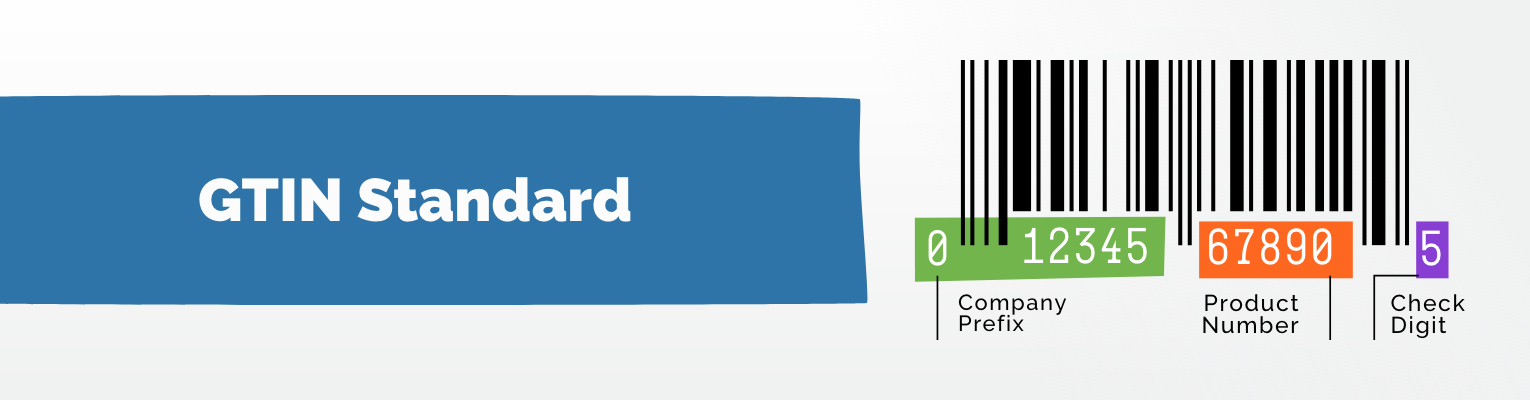
\includegraphics[width=0.8\textwidth]{./img/barcode_gtin12.jpg}
     \caption[GTIN-12 barcode]{\label{fig:barcorde} GTIN-12 barcode. }
\end{figure}

\subsubsection{GLN}
De GLN-code, ofwel het Global Location Number, is een unieke identificatiecode die wordt gebruikt om locaties te identificeren in de toeleveringsketen \autocite{GLN}.
Deze code is vergelijkbaar met de GTIN-code, maar wordt gebruikt voor locaties, de opbouw is ook gelijkaardig.
De GLN-code moet sinds 1 juli 2022 uniek zijn en mag niet hergebruikt worden voor andere locaties.
Eerst is er de bedrijfsprefix, daarna volgt het adresnummer en als laatste het controlecijfer.
Dit controlecijfer wordt op dezelfde manier berekend als bij de GTIN-code.
De bedrijfsprefix is een unieke code die wordt toegekend aan het bedrijf, deze code kan aangevraagd worden bij GS1. Het adresnummer is een unieke code die wordt toegekend aan de locatie, dit kan bijvoorbeeld een gebouw of een afdeling zijn.

\subsection{EPCIS-events}
Voor dit onderzoek wordt gebruikgemaakt van EPCIS (Electronic Product Code Information Services). Dit is een GS1-standaard die bedrijven in staat stelt om gebeurtenissen vast te leggen en te delen. 
Het biedt een gemeenschappelijk kader voor het vastleggen van het wat, wanneer, waar, waarom en hoe van gebeurtenissen die betrekking hebben op fysieke of digitale objecten. 
Deze waarden zijn ontwikkeld door GS1 om gegevens over beweging, status en verandering van een item in de toeleveringsketen (supply chain) vast te leggen en te delen binnen en buiten het bedrijf \autocite{Devins}.
``Met behulp van deze waarden kunnen we real-life objecten omzetten in elektronisch opgeslagen informatie, waarna we dit kunnen communiceren met eindgebruikers, zegt \textcite{Devins}.

Door deze normen toe te passen, kan de traceerbaarheid van het product per proces gegarandeerd worden, inclusief de gewenste parameters die opgeslagen worden in ons grafiekmodel zoals tijd (wanneer) en temperatuur (hoe), waar nodig.
Voor het correct en volgens de normen opstellen van deze relaties bestaan er EPCIS-events. Dit is een referentielijst waarin verschillende acties vooraf zijn bepaald.
Hierin staan bijvoorbeeld acties zoals \texttt{add}, \texttt{delete} en \texttt{update}, die gebruikt worden om de data te structureren en relaties aan te maken \autocite{Byun2020}.
Met de actie \texttt{add} wordt er een relatie toegevoegd, bijvoorbeeld met het label \texttt{IS\_ASSOCIATED} en de tijdstempel van wanneer de associatie is aangemaakt.
Bijvoorbeeld, als er een machine is met een bepaalde motor, zullen de machine en de motor gekoppeld zijn met een EPCIS-event \texttt{IS\_ASSOCIATED} die ook properties bevat zoals de tijdstempel van de associatie.
Bij deze actie worden ook properties toegevoegd in een event-lijst, daar wordt bepaald om welk soort event het gaat en worden eventuele extra parameters toegevoegd voor de relatie, zoals de tijd van het event.

In codefragment~\ref{fig:jsonld} is een voorbeeld te zien van een associatie-event tussen een machine en een component.

De belangrijkste voordelen volgens \textcite{GS12025} staan opgelijst in tabel~\ref{tab:epcis-voordelen}.
\begin{table}[H]
    \centering
     \begin{tabular}{lp{0.6\textwidth}}
          \toprule
          \textbf{Voordeel} & \textbf{Beschrijving} \\
          \toprule
          Verbeterde zichtbaarheid & Door het vastleggen en delen van gedetailleerde gebeurtenisgegevens kunnen bedrijven beter inzicht krijgen in de bewegingen en status van producten in de toeleveringsketen. \\
          \midrule
          Efficiëntieverbeteringen & Door het automatiseren van gegevensverzameling en -uitwisseling kunnen bedrijven operationele efficiëntie verbeteren en fouten verminderen. \\
          \midrule
          Naleving van regelgeving & EPCIS helpt bedrijven te voldoen aan wettelijke vereisten voor traceerbaarheid en rapportage. \\
          \midrule
          Betere samenwerking & Door het delen van gebeurtenisgegevens met partners kunnen bedrijven beter samenwerken en de toeleveringsketen optimaliseren. \\
          \bottomrule
     \end{tabular}
     \caption[Belangrijkste voordelen van EPCIS volgens GS1]{\label{tab:epcis-voordelen}}
\end{table}

\subsection{Schema.org}
Schema.org is een grote verzameling van gestructureerde data die entiteiten (knopen) en relaties kan weergeven \autocite{Douglas2023}.
GS1 en schema.org zijn complementair aan elkaar: GS1 richt zich op de identificatie en codering van producten, terwijl schema.org zich focust op de semantische betekenis van data.
In dit project worden objecttypen uit schema.org gecombineerd met concepten van GS1 om onze data gestructureerd en semantisch rijk te modelleren.
Met ``semantisch rijk'' wordt bedoeld dat de data meer betekenis krijgt. Zo wordt bijvoorbeeld de eigenschap \texttt{containedInPlace} van schema.org gebruikt om de relatie tussen een locatie en een asset te definiëren.
Van GS1 worden de EPCIS-events gebruikt om acties te definiëren die uitgevoerd worden op de data, zoals het toevoegen of verwijderen van een relatie.

Elke locatie krijgt een type, een label en extra properties, zoals een adres of een geografische locatie.
Dit type of ID kan bijvoorbeeld \texttt{Place} zijn voor een locatie of \texttt{Product} voor een asset.
Op de website van schema.org zijn alle mogelijkheden beschikbaar om data te structureren en te annoteren.

In codefragment~\ref{fig:jsonld} is een voorbeeld te zien van een JSON-LD-bestand met gegevens volgens schema.org in het eerste JSON-object.
In dit voorbeeld is Gent een locatie van het type \texttt{Place} met als \texttt{label} ``Gent''. De ouderknoop of \texttt{containedInPlace} is \texttt{null}, aangezien Gent de hoofdlocatie is.
Daarnaast is er te zien in het tweede JSON-object een EPCIS-document dat de associatie tussen twee fabrieken en Gent vastlegt.
De \texttt{parentID} is de locatie Gent en de \texttt{childEPCs} zijn de twee fabrieken die aan Gent zijn gekoppeld.
Het event \texttt{ADD} geeft aan dat er een associatie is toegevoegd tussen de fabrieken en Gent.
Het type associatie wordt bepaald door de eigenschap \texttt{epcis:AssociationEvent}.

\begin{listing}[H]
     \begin{minted}[fontsize=\scriptsize]{jsonld}
          {
          "@context": {
               "schema": "https://schema.org",
               "epcis": "https://ref.gs1.org/epcis/",
               "cbv": "https://ref.gs1.org/cbv/"
          },
          "@graph": [
               {
                    "@id": "123",
                    "@type": "Place",
                    "name": "Gent",
                    "label": "Gent",
                    "schema:containedInPlace": null,
                    "KEY": "VALUE"
               },
               {
                    "@type": "epcis:EPCISDocument",
                    "schemaVersion": "2.0",
                    "creationDate": "2025-03-19T17:40:54Z",
                    "epcis:EPCISBody": {
                         "epcis:EventList": {
                              "epcis:AssociationEvent": {
                                   "eventTime": "2025-03-19T17:40:54Z",
                                   "eventTimeZoneOffset": "+01:00",
                                   "parentID": ["Gent"],
                                   "childEPCs": [
                                        "fabriek 1",
                                        "fabriek 2"
                                   ],
                                   "event": "ADD",
                                   "disposition": "cbv:disp:active"
                              }
                         }
                    }
               }
          ]
          }
     \end{minted}
     \caption[Voorbeeld JSON-LD bestand]{\label{fig:jsonld}Voorbeeld van een JSON-LD bestand met locatiegegevens.}
\end{listing}

\section{Chatbot}{\label{sec:chatbot}}
De chatbot is een belangrijk onderdeel van ons project, aangezien het doorzoeken van de data zonder chatbot zeer tijdrovend en moeilijk is.
Dit zou eventueel kunnen gebeuren door zelf handmatig Gremlin-query's te schrijven, maar dit is niet efficiënt en vereist veel technische kennis van de gebruiker.
De chatbot zal ons helpen om de data snel en efficiënt te doorzoeken en de juiste informatie te vinden.

In deze thesis is de chatbot een REST-API die de vragen van de gebruiker kan beantwoorden op basis van de verzamelde data.
Wat een REST-API is en hoe deze werkt, is al eerder besproken in sectie~\ref{sec:restapi}.
Om de vragen te beantwoorden worden twee verschillende modellen gecombineerd, namelijk Phi-4 en CodeLLaMA. 
Zoals eerder besproken in sectie~\ref{sec:phi4} is Phi-4 een large language model dat zeer goed is in het verwerken van natuurlijke taal en lichtgewicht is.
Daarnaast is er ook CodeLLaMA, dit model is specifiek ontworpen voor het genereren van code en kan goed omgaan met de Gremlin-query's.
Om te zorgen dat de chatbot met beide modellen kan werken, zijn er een aantal stappen ondernomen.

Eerst en vooral is de chatbot zelf in NodeJS opgezet, waarbij een runtime wordt aangemaakt die bereikbaar is via bijvoorbeeld Postman.
Vervolgens wordt er via deze JavaScript-runtime een JSON-object met de vraag aangemaakt, zoals in codefragment~\ref{fig:userQuestion} te zien is.
Dit JSON-object (de vraag) wordt dan teruggestuurd naar JavaScript, die op zijn beurt een Python-script aanroept voor het genereren van een query.
Er wordt gebruikgemaakt van Python omdat AI-modellen vaak beter ondersteund worden in Python en er veel bibliotheken beschikbaar zijn voor het werken met AI-modellen.

\begin{listing}[H]
     \begin{minted}{json}
          {
               "vraag": "Wat is de status van machine 1?",
          }
     \end{minted}
     \caption[Voorbeeld JSON vraag]{\label{fig:userQuestion}Voorbeeld van vraag in JSON.}
\end{listing}

\subsection{Retrieval Augmented Generation}
Om onze chatbot te optimaliseren wordt er gebruikgemaakt van RAG (Retrieval Augmented Generation).
Dit is een techniek die het mogelijk maakt om de chatbot te laten leren van de data die is verzameld in ongestructureerde teksten, databases of andere bronnen~\autocite{Zeichick2023}.
Hierdoor kan de chatbot beter begrijpen wat er van hem verwacht wordt en hoe hij de vragen moet beantwoorden zonder het model volledig te hertrainen.
Dit is een low-level, maar veelgebruikte oplossing, die snel en flexibel bruikbaar is door documenten of context extra toe te voegen.

Hierbij wordt een simpel tekstbestand met context aangemaakt, waarbij de nodige informatie wordt meegegeven, zoals wat de functie is van het AI-model en wat belangrijk is of niet.
Daarnaast zijn er ook een aantal voorbeeldvragen en -antwoorden toegevoegd via een JSON-bestand, die geïndexeerd worden in een Elasticsearch-cluster binnen de Docker-container, dit principe wordt besproken in~\ref{sec:Elasticsearch}.
Dit is een belangrijke stap, omdat de chatbot hierdoor beter kan begrijpen wat er van hem verwacht wordt en hoe hij de vragen moet beantwoorden.
Daarnaast is het belangrijk dat in de context wordt meegegeven dat hij geen tekst of codeblokken mag genereren, maar enkel en alleen de query mag teruggeven.
Hiervoor is ook een veiligheidsmechanisme gecodeerd dat ervoor zorgt dat de query geen codeblok is zoals in markdown, door de backticks te verwijderen.
Dit gebeurt door de query te filteren op backticks en alles voor en na deze backticks te verwijderen (voorbeeldcode in figuur~\ref{fig:cleanQuery}). Doordat LLMs vaak codeblokken genereren in markdown, is dit een belangrijke, maar eenvoudige stap.
Dit is een belangrijke stap aangezien deze query direct moet worden geïmplementeerd in de database, wat betekent dat als er overige tekst of karakters in staan, het genereren zal mislukken door syntaxfouten.
Indien een query succesvol uitgevoerd is, wordt deze query ook opgeslagen in de JSON en toegevoegd aan de Elasticsearch-cluster.
Het is ook belangrijk dat hij de JSON-resultset met items kan omzetten naar natuurlijke taal en begrijpt wat er wel of niet meegegeven mag worden.
Als voorbeeld is het zo dat er in het antwoord soms databaseperformantiemetingen meegegeven worden die niet in het antwoord mogen staan voor de gebruiker.

Door al deze ``vereisten'' als context mee te geven aan de chatbot, kan hij beter begrijpen wat er van hem verwacht wordt en hoe hij de vragen moet beantwoorden.

\begin{listing}[H]
     \begin{minted}{js}
          query = query.replace("gremlin", "").replace("```", "").strip()
          // ```gremlin g.V().has('name', 'motor')``` ==> g.V().has('name', 'motor')
     \end{minted}
     \caption[Voorbeeld van het schoonmaken van de query]{\label{fig:cleanQuery}Voorbeeld van het schoonmaken van de query.}
\end{listing}

\subsection{Elasticsearch}\label{sec:Elasticsearch}
Elasticsearch is een open-source zoek- en analysetool die gebruikt wordt om snel door grote hoeveelheden data te zoeken en deze te analyseren~\autocite{Elastic2025}.
Het is gebouwd op Apache Lucene en werkt via een REST-API, waardoor het makkelijk te integreren is en tegelijk krachtig genoeg om schaalbaar met data om te gaan.

Omdat Elasticsearch werkt met een gedistribueerde architectuur, kan het data en rekenkracht verdelen over meerdere servers.
Dat zorgt voor betere prestaties en maakt het mogelijk om makkelijk op te schalen wanneer er meer data bijkomt.
In deze thesis gebruik ik Elasticsearch om JSON-data rond Gremlin-query's op te slaan in een index, zodat ik deze snel kan doorzoeken.

Een groot voordeel van Elasticsearch is dat het data indexeert en opdeelt in tokens.
Dat is handig bij het stellen van vragen, omdat het minder strikt kijkt naar de exacte volgorde van woorden~\textcite{Oers2025}.
Zo kunnen ook vragen die niet letterlijk in de dataset staan, maar er wel op lijken, toch goede resultaten opleveren.

Naast tokenisatie maakt Elasticsearch ook gebruik van een omgekeerde index (inverted index).
Dit is een datastructuur die het toelaat om supersnel op te zoeken welke documenten bepaalde termen bevatten~\autocite{Brimley2023}.
In het volgende hoofdstuk leg ik dieper uit hoe tokenisatie en de omgekeerde index precies werken in Elasticsearch.

Om een Gremlin-query te genereren, gebruik ik een aanpak die ik beschrijf als een hybride Elasticsearch-integratie.
Meer uitleg daarover staat in sectie~\ref{sec:hybride-elasticsearch}.

Voor deze thesis gebruik ik de Elasticsearch Python-client in versie \texttt{8.12.0}, omdat deze stabiel is en alles ondersteunt wat ik nodig heb.
De eerste tests met versie \texttt{9.0} gaven problemen, omdat er op dat moment nog geen Python-client beschikbaar was voor die versie.


\subsubsection{Tokenisatie}
Tokenisatie is het proces waarbij een tekst wordt opgesplitst in kleinere stukjes (meestal woorden) die vervolgens in een zogenaamde \emph{token stream} terechtkomen~\autocite{Elastic}.
Zo'n token stream is eigenlijk gewoon een array met alle woorden uit de tekst, en deze wordt gebruikt om makkelijker te kunnen zoeken naar een passend antwoord.

Zowel de vraag van de gebruiker als de bestaande vragen in de Elasticsearch-cluster worden op deze manier getokeniseerd.
De \emph{vraag} is dus wat de gebruiker intypt, en de \emph{cluster} is de verzameling van alle eerder opgeslagen vragen in Elasticsearch.

Door de tokens van de vraag en de tokens uit de cluster met elkaar te vergelijken, kan er bepaald worden hoe goed ze overeenkomen.
Op basis daarvan (en met behulp van een ingestelde drempelwaarde (threshold)) kan er worden vastgesteld welke opgeslagen vraag het meest relevant is, en dus de beste match vormt.
In figuur~\ref{fig:invertedIndex} is een voorbeeld te zien van hoe tokenisatie werkt in Elasticsearch.

\subsubsection{Omgekeerde index}
De omgekeerde index (of inverted index) is een lijst van alle tokens die in een vraag voorkomen. Deze tokens krijgen in de omgekeerde index één of meer ID's toegewezen~\autocite{Vatsya2024}.
Deze ID's zijn unieke identificaties die verwijzen naar de vraag waarin de token voorkomt. Hierdoor wordt er enorm snel gezocht naar de juiste vraag en wordt deze teruggeven aan de gebruiker.

De relevantiescore van een vraag wordt berekend op basis van TF (term frequency) en IDF (inverse document frequency).
Dit betekent dat hoe vaker en hoe zeldzamer een token in een vraag is, hoe hoger de score zal zijn en dus hoe relevanter de vraag is.

In fragment~\ref{fig:invertedIndex} is een voorbeeld te zien van een zin die is omgezet naar een omgekeerde index.
Daar zal voor de vraag \emph{``Toon alle machines in Gent''} gekozen worden voor de query die hoort bij \emph{``Geef alle machines in Gent''}.
Dit komt omdat de frequentie van de tokens ``machines'' en ``Gent'' in de vraag hoger is dan die van de andere tokens.

\begin{listing}[H]
     \begin{minted}{text}
          {
              Document 1: "Geef alle machines in Gent"
              Document 2: "Toon alle motoren in Antwerpen"

              tokens: ['Geef', 'alle', 'machines', 'in', 'Gent', 'Toon', 'motoren', 'Antwerpen']
               inverted index: {
                    'Geef': [1],
                    'alle': [1, 2],
                    'machines': [1],
                    'in': [1, 2],
                    'Gent': [1],
                    'Toon': [2],
                    'motoren': [2],
                    'Antwerpen': [2]
               }
          }
     \end{minted}
     \caption[Voorbeeld inverted index]{\label{fig:invertedIndex}Voorbeeld van een inverted index.}
\end{listing}

\subsubsection{Hybride Elasticsearch-integratie voor querygeneratie}{\label{sec:hybride-elasticsearch}}
De integratie van alleen Elasticsearch is niet voldoende om de chatbot robuust te laten functioneren.
Doordat Elasticsearch alleen de vragen indexeert en doorzoekt, is het niet in staat om de vragen te begrijpen en om te zetten naar Gremlin-query's.
Daarom wordt er gebruikgemaakt van een hybride integratie van Elasticsearch, waarbij de resultaten van Elasticsearch gebruikt worden om een query te laten genereren.

Door de score van Elasticsearch te gebruiken, kan de chatbot bepalen welke vraag het meest relevant is voor de gestelde vraag.
Als een vraag een score hoger dan 15 heeft, wordt de bijbehorende query gebruikt om de data op te halen.

Als de score hoger is dan 12, maar lager dan 15, wordt de vraag nog eens bekeken door het Large Language Model (CodeLLaMA) met de vorige best passende query (hoogste score).
Door deze extra stap kan de chatbot mogelijke aanpassingen doen aan de query, waardoor hij beter in staat is om de juiste query te genereren.
Met deze foutieve query en de context van het contextbestand kan de chatbot proberen om een nieuwe query te genereren die beter aansluit bij de vraag van de gebruiker.
In figuur~\ref{fig:chatbot_workflow} is de workflow te zien van de hybride integratie van Elasticsearch voor querygeneratie.
Daarnaast is er in codefragment~\ref{fig:elasticsearchQuery} een voorbeeld te zien van de Elasticsearch-query die wordt gebruikt om de vragen te doorzoeken.

\begin{listing}[H]
     \begin{minted}{python}
          if response["hits"]["hits"]:
             best_hit = response["hits"]["hits"][0]
             score = best_hit["_score"]
             if score >= 15:
                 query = best_hit["_source"]["antwoord"]
                 return query
             else if score >= 12:
                 previous_query = best_hit["_source"]["antwoord"]  # Sla de vorige query op
                 if previous_query:
                     query = generate_query_from_llm(question, context, previous_query, error)
                     return query
     \end{minted}
     \caption[Voorbeeld Elasticsearch query bepalen]{\label{fig:elasticsearchQuery}Voorbeeld van hoe we een Elasticsearch query bepalen.}
 \end{listing}

\subsection{Docker}
Docker is een open-source platform dat het mogelijk maakt om applicaties te ontwikkelen en uit te voeren in containers~\autocite{docker2025}.
In deze thesis wordt Docker gebruikt om de verschillende componenten van de chatbot te isoleren en te beheren.
Daarnaast zorgt Docker ervoor dat de omgeving van de applicatie consistent is, ongeacht waar deze wordt uitgevoerd.
Hierdoor kan de applicatie eenvoudig worden geïmplementeerd en geschaald, zonder zorgen over de onderliggende infrastructuur.

Docker maakt gebruik van images die in containers worden uitgevoerd. Elke image kan meerdere containers bevatten met hun eigen eigenschappen.
Docker is ook sneller en performanter dan traditionele virtuele machines, omdat het geen volledige besturingssystemen hoeft te emuleren.
Met behulp van Docker kan de chatbot eenvoudig worden geïmplementeerd en laten communiceren met andere componenten, zoals de Ollama-modellen en Elasticsearch.

\subsubsection{Docker images}
Docker-images vormen de basis van Docker-containers en bevatten alles wat nodig is om de applicatie uit te voeren~\autocite{Schmitt2024}.
Voor deze thesis is er een Dockerfile opgesteld die de basisimage bevat en de benodigde dependencies installeert.
In figuur~\ref{fig:dockerfile} is een voorbeeld te zien van de Dockerfile voor NodeJS die wordt gebruikt om de chatbot te bouwen.

\subsubsection{Docker containers}
Docker-containers zijn geïsoleerde processen die gebaseerd zijn op een Docker-image, zonder effect op andere delen van het systeem~\textcite{Schmitt2024}.
Zo is er bijvoorbeeld een container voor de chatbot, een container voor Elasticsearch en een container voor de Ollama-modellen, die eenvoudig via een API kunnen worden aangeroepen en onderling kunnen communiceren.

\subsubsection{Docker-compose}
Om alle containers in één keer op te starten en te beheren, wordt gebruikgemaakt van Docker Compose~\autocite{docker2025}.
In figuur~\ref{fig:Docker-compose} is een voorbeeld te zien van een Docker Compose-bestand dat gebruikt is om de verschillende containers op te starten.
Het gebruik van Docker Compose is vooral geschikt op kleine schaal. Voor schaalvergroting naar een productieomgeving kan Kubernetes worden ingezet.
Kubernetes zorgt ervoor dat containers automatisch worden geschaald en beheerd.
